\chapter{Executive Summary}
\label{ch:intro}


%%%%%%%%%%%%%%%%%%%%%%%%%%%%
\section{The DUNE Near Detector Science Program}
\label{intro:science}
%\fixme{I like this title better than just ``Physics''}
The primary goal of the \dword{dune} 
\dword{nd} is to perform critical measurements near the \dword{lbnf} neutrino beam prior to the onset of neutrino oscillation effects to minimize the systematic uncertainties in  the long baseline neutrino oscillation measurements. Data from the \dword{nd} provides information on the neutrino flux, %their interaction 
the neutrino interactions on argon nuclei, and the response of the detector to the particles that emerge from the interaction necessary to accurately predict the observed spectrum of each neutrino species at the \dword{fd}
in the presence of neutrino oscillations and backgrounds. The \dword{lbl} %long baseline 
neutrino oscillation measurement is in effect an integrated measurement between \dword{nd} and \dword{fd}, where the \dword{fd} spectrum predicted using data from \dword{nd} as a function of the neutrino oscillation parameters is compared to the observations at \dword{fd} to extract the neutrino oscillation parameters. To this end, the \dword{nd} must provide sufficient information through its measurements to minimize the systematic uncertainties in the \dword{fd} which would otherwise suffer large uncertainties if otherwise unconstrained predictions based on {\em ab initio} simulations are used.

The requirements and design of \dword{nd} are driven by the needs of the \dword{lbl} %long baseline 
neutrino oscillation measurements, and therefore are tightly coupled to the  expected measurement capabilities and systematic uncertainties at the \dword{fd}.

Except where explicitly noted, we assume that any discussion of neutrinos also refers to antineutrinos, including data-taking with \dword{lbnf} in both neutrino-enhanced forward horn current (FHC) and antineutrino-enahced (RHC) modes.

%%%%%%%%%%%%%%
\subsection{Other Physics}
\label{intro:science:other}
The intense neutrino beam produced by \dword{lbnf} can support a wide range of physics measurements and studies using \dword{nd}, including:
\begin{itemize}
    \item {\bf Neutrino-nucleus interactions studies:} A large variety of interactions can be studied due to the reconstruction capabilities of the detector, the wide energy range, assortment of materials and nuclear targets with high statistics. 
    \item {\bf Short baseline neutrino oscillations:} Exotic neutrino states with large mass splittings may induce neutrino oscillations on a short distance scale which may be visible in the \dword{nd} %near detector 
    system.
    \item {\bf Exotic physics  :} The \dword{lbnf} neutrino beam may produce exotic particles in the primary proton interactions on the target, the subsequent decay of secondary particles, or through neutrino interactions which may be detectable through their interaction or decay in the near detector system.
\end{itemize}
Neutrino-nucleus interaction studies at \dword{nd}, particularly on argon, are intimately connected to its primary role in the long baseline neutrino oscillation program, but differ in providing independent measurements on the property of these interactions rather than integrating them into the extraction of neutrino oscillation parameters. Due to this difference, the channels of interest and measurement strategy may differ considerably between in the two cases. Neutrino-nucleus interaction measurements also support other DUNE physics goals, such as the search for nucleon decay in the \dword{fd} or exotic particle searches in either detector, where they may improve the estimate of backgrounds arising from neutrino interactions.

The requirements of these additional physics programs do not explicitly drive the design of \dword{nd} but the extensive capabilities needed to deliver the requirements for the long baseline measurements will enable a compelling program in these other areas.

%%%%%%%%%%%%%%
\subsection{Neutrino Oscillations}
\label{intro:science:nuosc}
%Relatively standard introduction . . .  follow TDR/ND CDR
The quantum mechanical mixing of neutrino flavor and mass states which manifests in a time dependence to the flavor content of a neutrino, called neutrino oscillations. Since neutrinos are typically produced and interact in flavor states via the weak interaction, this mixing allows the possibility that a neutrino is produced in one flavor and interacts in a different flavor. This probability oscillates as a function of $L/E$, where $L$ is the distance between the production and interaction of the neutrino and $E$ is its energy. The frequency of these oscillations in $L/E$ are set by the differences squared mass eigenvalues ($\Delta m_{ij}^2$) and the amplitudes by the mixing matrix $U_{ij}$ which relates the mass and flavor eigenstates of the neutrino.
\begin{itemize}
    \item 
\item $P(\nu_\mu\to\nu_e)$
\end{itemize}
.  ,  governed by the unitary mixing matrix relating the flavor and mass states and the mass splittings, 


%%%%%%%%%%%%%%
\subsection{Goals of Experiment}
\label{intro:science:goals}
Neutrino oscillations are measured by comparing the observed spectrum of the neutrino interactions observed at the \dword{fd} to the predicted spectrum, which results from a convolution over neutrino energy ($E_\nu$) of the following quantities:
\begin{itemize}
    \item $\Phi_\alpha(E_\nu)$: The initial flux and spectrum produced by the \dword{lbnf} beam in each flavor $\nu_\alpha$.
    \item $P(\nu_\alpha\to\nu_\beta,E_\nu)$: The probability for oscillation from the initial flavor $\nu_\alpha$ to the flavor $\nu_\beta$ due to neutrino oscillations, determined by the neutrino mass and mixing parameters.
    \item $\sigma_\beta(E_\nu)$: The modeling of the $\nu_\beta$ with energy $(E_\nu)$ on the argon nucleus including its interaction cross section and resulting outgoing particles.
%    \item $V\times n$: The number of argon target nuclei in the \dword{fd}
    \item $R_\beta(E_\nu)$:  The response of the detector to the interaction of $\nu_\beta$ to produce observables to select and kinematically characterize ({\em e.g.} reconstruct the neutrino energy) of a $\nu_\beta$ interaction. 
\end{itemize}
Assuming the $\Phi_\alpha$, $\sigma_\beta$, and $R_\beta$ are well-understood, the oscillation parameters governing $P(\nu_\alpha\to\nu_\beta)$ can be extracted. Figure \ref{fig:fd_nmu_nue}

Background
%Long baseline neutrino physics
%Emphasize multiparameter nature of the physics . . . . it’s not just about nue appearance, but in order to extract %parameters, including CPV correctly, DUNE must also be able to extract theta23, Dm2, etc. correctly.  Otherwise, DUNE’s %own measurements will either be in tension or biased.
%Explain the timeline for neutrino oscillation measurements .. . when do we expect to achieve certain milestones in %sensitivity/precision in order to set up staging discussion later.

\begin{dunefigure}[$\nu_\mu$,$\nu_e$ at \dword{fd}]{fig:fd_nmu_nue}
%  \centering
{Spectrum of $\nu_\mu$, $\nu_e$}
  \subfloat[][$E_{\rm rec}$]{
    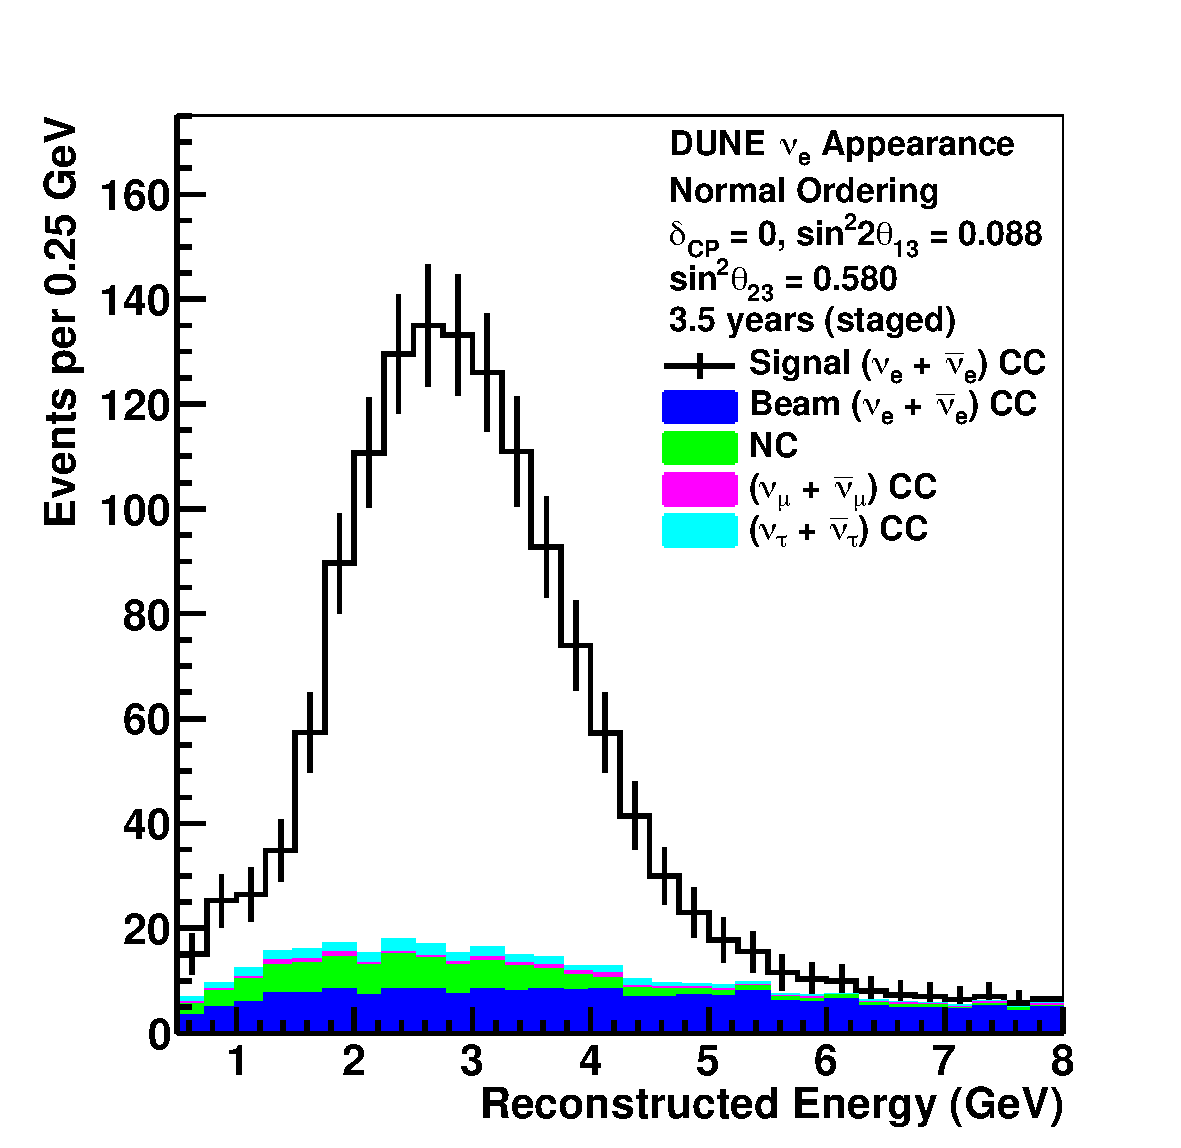
\includegraphics[width=0.45\textwidth]{spec_app_nu_no.pdf}

    %\label{fig:fd_nue}
  }
  \subfloat[][$E_{\rm proton}^{dep}$]{
    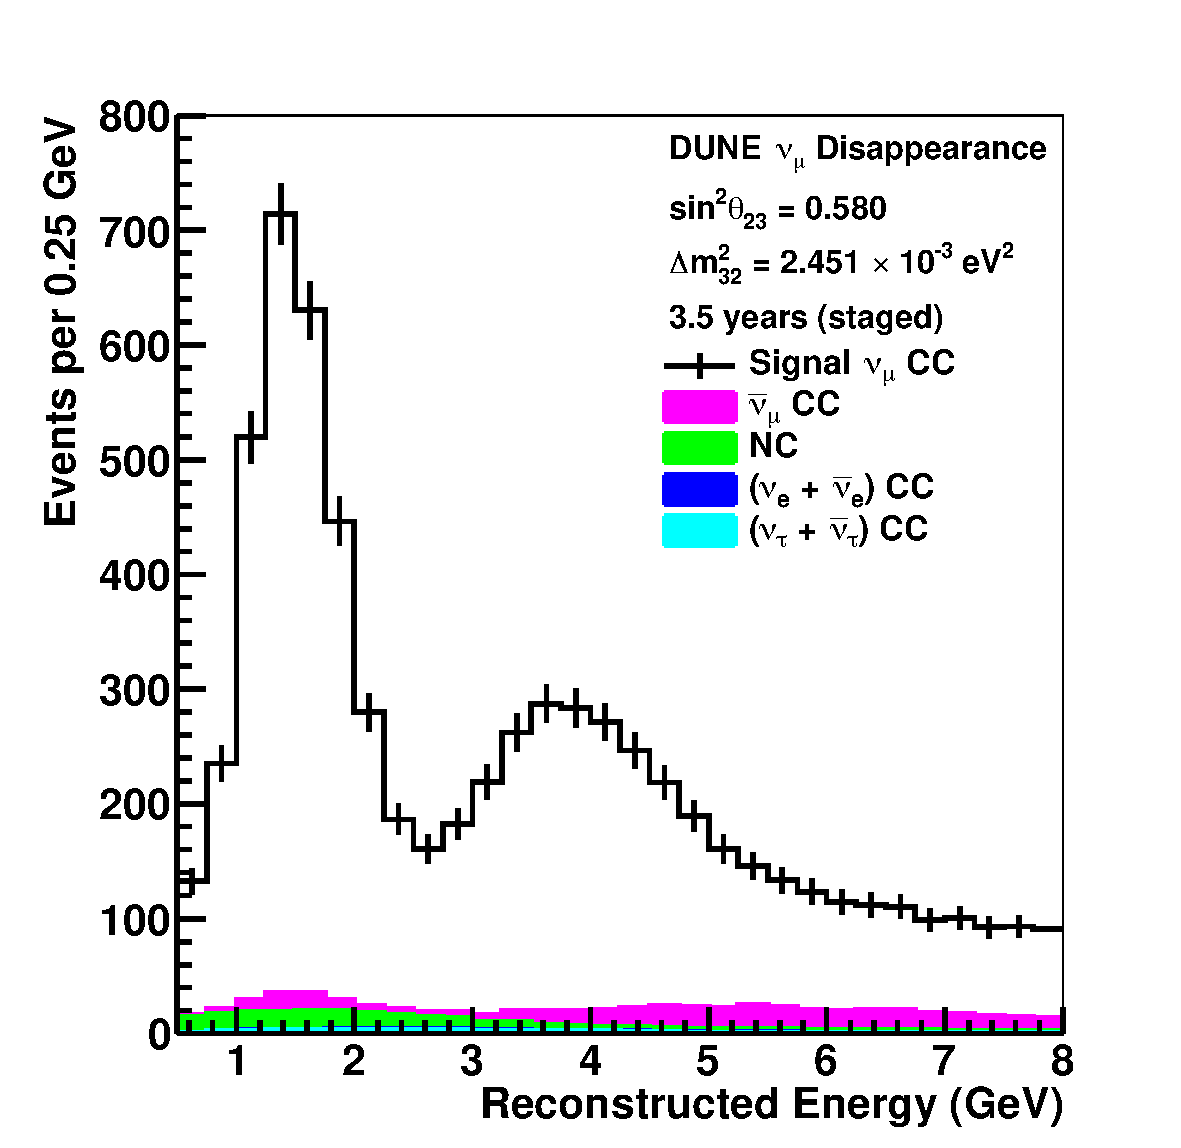
\includegraphics[width=0.45\linewidth]{spec_dis_nu_no.pdf}
    %\label{fig:fd_numu}
  }
\end{dunefigure}


%%%%%%%%%%%%%%
\subsection{Role of Near Detector}
\label{intro:science:role}


The role of the \dword{nd} in the long baseline neutrino oscillation analysis is summarized within the \dword{dune} Global Science Requirements:

{\em \dword{nd} measurements shall be of sufficient precision to ensure that when extrapolated to \dword{fd} to predict the \dword{fd} event spectra, the associated systematic error must not dominate the measurement precision.''}

To that end, the \dword{nd} must:
\begin{itemize}
    \item make measurements to constrain uncertainties in each component of the \dword{fd} prediction mentioned above, namely the initial neutrino fluxes $\phi_\alpha$, the neutrino interaction modeling $\sigma_\beta$, and the detector response $R_\beta$, so that in their total impact in predicting the \dword{fd} event spectra is less than the statistical uncertainty in the \dword{fd}. 
    \item have measurement capabilities sufficiently robust to mitigate unexpected sources of uncertainty in any part of the prediction. 
\end{itemize}

We summarize several key challenges which drive the requirements for \dword{nd} to fulfill these roles.

%%%%%%%%%%%%%%
\subsection{Requirements} %% Anne added 11/10
\label{intro:science:reqs}

% N.B. This file is generated, any edits may be lost.
\begin{footnotesize}
\begin{longtable}{p{0.12\textwidth}p{0.18\textwidth}p{0.17\textwidth}p{0.25\textwidth}p{0.16\textwidth}}
\caption{Specifications for ND-OVERARCH \fixmehl{ref \texttt{tab:spec:nd-overarch}}} \\
  \rowcolor{dunesky}
       Label & Description  & Specification \newline (Goal) & Rationale & Validation \\  \colhline

\newtag{ND-OVERARCH-01}{ spec:predict-the-observed-neutrino-spectrum-at-the-fd }  & Predict the observed neutrino spectrum at the FD  &  overarching requirements do not have values \newline () &  In combination with available external information, the long baseline analysis requires that we predict the number, spectrum, and flavor of neutrinos observed at the far detector, as well as backgrounds, along with any other information about these events that are used in the analysis. &   \\ \colhline
\newtag{ND-OVERARCH-02}{ spec:transfer-measurements-to-the-fd }  & Transfer measurements to the FD  &  None \newline () &  The ND must be able to measure interactions on a Ar target, and furthermore transfer observables as they would be seen in the FD LArTPCs. The transfer must be performed accounting for uncertainties arising from detector modelling, including thresholds, efficiencies, purities, and resolution in the context of observables that are used in the far detector, the neutrino interaction model, the flux, as well as the differing operating conditions in the near and far site (cosmic rate, beam interaction rate/backgrounds, etc.). &   \\ \colhline
\newtag{ND-OVERARCH-03}{ spec:constrain-the-cross-section-model }  & Constrain the cross section model  &  None \newline () &  The FD response couples the modelling of outgoing particles in nu-Ar interactions in terms of the mulitplicity, topology, and kinematics, to the ability to reconstruct these  particles. The near detector must sufficiently measure and constrain the uncertainties in this modelling to minimize their impact on the oscillation measurement. &   \\ \colhline
\newtag{ND-OVERARCH-04}{ spec:measure-the-neutrino-flux }  & Measure the neutrino flux  &  None \newline () &  The ab initio prediction of the neutrino flux is based on Monte Carlo simulation which has uncertainties arising from particle production, beam optics, operational variation, etc. that must be verified and constrained by the near detector. Secondary components of the flux give rise to irreducible backgrounds in the FD which must be constrained &   \\ \colhline
\newtag{ND-OVERARCH-05}{ spec:obtain-measurements-with-different-fluxes }  & Obtain measurements with different fluxes  &  None \newline () &  The flux and spectrum of neutrinos can be varied by moving the detectors off-axis or changing the horn currents. The near detector must verify that its model predictions and constraints are robust against these variations, which would otherwise give rise to degenerate tunings that bias the FD predictions and the resulting oscillation parameters. &   \\ \colhline
\newtag{ND-OVERARCH-06}{ spec:monitor-time-variations-of-the-neutrino-beam }  & Monitor time variations of the neutrino beam   &  None \newline () &  The flux and spectrum of neutrinos delivered by the beam can vary due to operational variations as well as unexpected component variances or failures. The near detector must detect such variations in such a way that they can be identifed promptly and any compromised beam delivery is minimized. &   \\ \colhline
\newtag{ND-OVERARCH-07}{ spec:operate-in-high-rate-environment }  & Operate in high rate environment  &  None \newline () &  The ND operates in a significantly different environment from the FD, with  higher cosmic ray rates as well as pile up of beam-related activity (including other neutrino interactions). The ND must be robust against this additional activity in fulfilling the other overarching requirements. &   \\ \colhline

\label{tab:specs:nd-overarch}
\end{longtable}
\end{footnotesize}


% N.B. This file is generated, any edits may be lost.
\begin{footnotesize}
\begin{longtable}{p{0.12\textwidth}p{0.18\textwidth}p{0.17\textwidth}p{0.25\textwidth}p{0.16\textwidth}}
\caption{Specifications for ND-MEAS \fixmehl{ref \texttt{tab:spec:nd-meas}}} \\
  \rowcolor{dunesky}
       Label & Description  & Specification \newline (Goal) & Rationale & Validation \\  \colhline

\newtag{ND-M3}{ spec:nu-e-scatt-flux }
  & Nu-electron scattering flux measurements 
  &  The ND must measure the flux with $\nu$-e scattering, a standard candle that provides a normalization measurement. 
  &  $\nu$-e elastic scattering has a very well known but tiny cross section. With a sufficiently large sample of cleanly idenified events, the flux can be measured precisely and without the model dependence present in $\nu$-nucleus scattering.
  &   \\ \colhline
\newtag{ND-M8}{ spec:tms-on-axis-numu-rate }
  & TMS: On-axis numu interaction rate
  &  The ND must have a component that remains on-axis where beam monitoring is most sensitive in order to identify a sufficient number of $\nu_\mu$ CC events to satisfy the beam monitoring requirements.  
  &  Since the oscillation measurements are made with the on-axis flux and measurements are required off-axis, a component of the near detector must remain on-axis to perform the beam monitoring masurements.
  &   \\ \colhline
\newtag{ND-M10}{ spec:ext-bkgd-meas }
  & External background measurements
  &  The ND must be able to measure external backgrounds, which include cosmic rays and beam-induced activity. 
  &  Due to the shallow site and the intensity of the neutrino beam, the ND operates in an environment with cosmic rays and a high level of beam-induced background activity. In order to verify that these backgrounds are correctly accounted for and modeled, the ND must be able to measure them. 
  &   \\ \colhline
\newtag{ND-M6}{ spec:beam-nue-bkgd }
  & Intrinsic beam nue measurements
  &  The ND must measure and validate the modelling of intrinsic beam $\nu_e$, an irreducible background. 
  &  Intrinsic beam $\nu_e$ are irreducible and dominant background in the $\nu_e$ appearance analysis. This component must be measured and its modeling verified.
  &   \\ \colhline
\newtag{ND-M5}{ spec:wrong-sign-meas }
  & Wrong-sign interaction measurements
  &  The ND must measure and validate the modelling of wrong-sign interactions that dilute the oscillation asymmetries at the FD. 
  &  The neutrino oscillation measurements rely on measuring neutrino and antineutrino oscilllations separately in FHC/RHC operation. Particularly in RHC, there is a large component of numu events that will partially ``wash out'' oscillation asymmetries and is irreducible at the FD. This component must be measured and its modeling verified to verify backgrounds and the right-sign flux.
  &   \\ \colhline
\newtag{ND-M1}{ spec:ndlar-reco-like-fd }
  & ND-LAr reconstruction comparable to FD
  &  The ND must have a LArTPC with reconstruction capabilities comparable/exceeding the far detector in order to effectively transfer measurements. 
  &  The ND must observe and reconstruct the products of neutrino interaction such that we can infer how those interactions would appear in the far detector. The interactions must be observed in liquid argon and without gaps in acceptance that would leave phase space of neutrino energy and energy transfer uncovered. Due to the close coupling of detector effects with neutrino event modellling, ND measurements with a LArTPC must be made to ensure that the overall modelling of the interaction and detector response are accurate.
  &   \\ \colhline
\newtag{ND-M2}{ spec:ndlar-recoil-meas }
  & ND-LAr recoil particle measurements
  &  The ND must measure outgoing recoil particles ($\pi$, p, $\gamma$) in $\nu$-Ar interactions with uniform acceptance, lower thresholds than a LArTPC, and with minimal secondary interactions to ensure that sensitive phase space is properly modeled. 
  &  ND-LAr will have several challenges in addressing systematics: non-uniform acceptance  (azimuthal, against important observables such as $E_\nu$ and energy transfer, etc.); significant secondary interactions, and high detection thresholds for outgoing particles due to the density of LAr. Measurements with a uniform acceptance will verify that the modelling is accurate, while the lower thresholds and minimal secondary interactions will allow the multiplicity and kinematics of outgoing hadrons from the $\nu$-Ar interaction to be  compared against the model in detail.
  &   \\ \colhline
\newtag{ND-M4}{ spec:low-nu-flux-spectrum }
  & Low-nu flux spectrum measurements
  &  The ND must identify/measure low recoil energy events that have flat energy dependence in order to measure the neutrino flux spectrum (``low-nu'' method). 
  &  The $\nu$-e elastic scattering measurement has weak constraints on the shape of the spectrum due to beam divergence. An accurate understanding of the shape is important in fully utilizing the spectral shape of the oscillations. The low-nu method allows the shape to be constrained for $E_\nu >$\SI{1}{GeV} with \SI{100}{MeV} recoil threshold.
  &   \\ \colhline
\newtag{ND-M9}{ spec:tms-on-axis-bm-monitor }
  & TMS: On-axis beam monitoring
  &  The ND must use on-axis spectrum information to detect representative changes in the beamline. 
  &  Rate information alone is insufficient to detect some beam variations that will impact the oscillation analysis. The beam monitoring must use spectrum information from muon/neutrino energy. 
  &   \\ \colhline
\newtag{ND-M7}{ spec:prism-off-axis-meas }
  & PRISM: Off-axis measurements
  &  The ND must be able to move off the beam axis to take data with neutrino spectra varying across the region of interest for neutrino oscillation measurements. 
  &  Mismodelling that impacts the $E_\nu$ reconstruction directly impacts neutrino oscillation measurements, since this is a key observable. Varying the incident flux by placing ND-LAr (+TMS/ND-GAr) at different off-axis positions allow the modeling of the reconstruction to be explicitly verfied. The upper limit is set by the variation that can be probed by this method. The lower limit set by the range over which DUNE will perform long-baseline neutrino oscillation measurements.
  &   \\ \colhline

\label{tab:specs:nd-meas}
\end{longtable}
\end{footnotesize}


% N.B. This file is generated, any edits may be lost.
\begin{footnotesize}
\begin{longtable}{p{0.12\textwidth}p{0.18\textwidth}p{0.17\textwidth}p{0.25\textwidth}p{0.16\textwidth}}
\caption{Specifications for ND-CAP \fixmehl{ref \texttt{tab:spec:nd-cap}}} \\
  \rowcolor{dunesky}
       Label & Description  & Specification \newline (Goal) & Rationale & Validation \\  \colhline

\newtag{ND-C1}{ spec:ndlar-reco-nd-vs-fd }
  & ND-LAr particle reconstruction performance
  &  In order to effectively translate measurements to the FD, ND-LAr must be able to reconstruct particles from neutrino events with comparable/better performance than the FD 
  &  
  &  Simulation \\ \colhline
\newtag{ND-C1.1.1}{ spec:ndlar-nue-id }
  & ND-LAr electron neutrino identification
  &  ND-LAr must identify and reconstruct  $\nu_e$ events as well as FD 
  &  ND-LAr nue identification and reconstruction is needed to verify the modelling of the $\nu_e$  flux and cross section, as well as the respone of the FD
  &  Simulation \\ \colhline
\newtag{ND-C1.1.2}{ spec:ndlar-numu-id }
  & ND-LAr muon neutrino identification
  &  ND-LAr must identify and reconstruct  $\nu_\mu$ events as well as FD 
  &  ND-LAr numu identification and reconstruction is needed to verify the modelling of the  $\nu_\mu$ flux and cross section, as well as the respone of the FD
  &  Simulation \\ \colhline
\newtag{ND-C1.1.3}{ spec:ndlar-cont-particle-reco }
  & ND-LAr contained particle reconstruction
  &  Contained particles emerging from ND-LAr should be detected as well as FD. 
  &  ND-LAr particle reconstruction is needed to verify and correct modeling to the extent the the FD observes the corresponding particles.
  &  Simulation \\ \colhline
\newtag{ND-C1.1.4}{ spec:ndlar-limit-uncont-had }
  & ND-LAr limit for uncontained hadron shower
  &  Event topologies/kinematics where no geometric configuration would contain the hadron shower must be limited. 
  &  Uncovered phase space is effectively completely unconstrained by ND-LAr measurements and thus will have a large uncertainty in their contribution to FD distributions. 
  &  Simulation \\ \colhline
\newtag{ND-C1.2.1}{ spec:ndlar-stat-uncert-nue }
  & ND-LAr  statistical uncertainty in electron neutrino measurement
  &  ND-LAr must collect sufficient statistics to allow $<2\%$ statistical uncertainty in the $\nu_e$ measurement 
  &  In order to make a precise measurement, high statistics in this low-cross section process is needed
  &  Simulation \\ \colhline
\newtag{ND-C1.2.2}{ spec:ndlar-id-recoil-e }
  & ND-LAr identification of recoil electron
  &  ND-LAr must be able to identify the recoil electron, distinguish it from other particles ($\mu, \gamma, \pi^0$), and also from $\nu_e$ -CC 
  &  In oder to make a precise measurement, an efficient and pure selection is needed 
  &  Simulation \\ \colhline
\newtag{ND-C1.2.3}{ spec:ndlar-e-energy-res }
  & ND-LAr electron energy resolution
  &  Energy resolution is needed to identify the forward $\nu_e$  events and measure its kinematics 
  &  Both the electron energy and angle are needed in separating this process from the background
  &  Simulation \\ \colhline
\newtag{ND-C1.2.4}{ spec:ndlar-e-ang-res }
  & ND-LAr electron angular resolution
  &  A tight cut on forward electrons is needed to identify $\nu_e$  events 
  &  Both the electron energy and angle are needed in separating this process from the background
  &  Simulation \\ \colhline
\newtag{ND-C1.2.5}{ spec:ndlar-vtx-thresh }
  & ND-LAr vertex activity threshold
  &  Identifying vertex activity near the electron vertex is necessary to reject backgrounds 
  &  $\nu_e$-CC and other backgrounds give rise to hadronic activity near the vertex that is not present for $\nu_e$ elastic events
  &  Simulation \\ \colhline
\newtag{ND-C1.3.1}{ spec:ndlar-scint-time-res }
  & ND-LAr scintillation timing resolution
  &  Scintillation timing is required to set the $t_0$ for the charge readout and to separate event pileup 
  &  The charge readout of ND-LAr occurs on the time scale of ms and does not provide an absolute reference ($t_0$). This is too long to isolate activity from the beam and  obscures the (absolute) coordinate along the drift axis.  The optical detection of scintillation photons must provide both $t_0$ and isolation of the activity from O(100) events spread within the beam delivery window of $\sim$\,\SI{10}{\micro\s}. 
  &   \\ \colhline
\newtag{ND-C1.3.2}{ spec:ndlar-intermod-scint-time }
  & Scintillation timing synchronization between ND-LAr modules
  &  Timing between modules must be synchronized in order to seamlessly integrate activity observed in the separate modules. 
  &  Time  synchronization betweem modules must be comparable to the scintillation timing resolution in order to ensure that event reconstruction across modules is not compromised.
  &   \\ \colhline
\newtag{ND-C2.1}{ spec:tms-ndgar-mu-acc }
  & TMS and ND-GAr muon acceptance
  &  TMS/ND-GAr must detect and analyzes muons exiting the ND-LAr without a gap in phase space coverage 
  &  This completes ND-C1.2 and complements ND-C1.3 by providing the corresponding muon acceptance at higher momentum.
  &  Simulation \\ \colhline
\newtag{ND-C2.2}{ spec:tms-ndgar-mu-res }
  & TMS and ND-GAr momentum resolution
  &  TMS/ND-GAr must measure the muon momentum at least as accurately as the FD 
  &  This completes ND-C1.2 by providing the corresponding muon kinematic reconstruction
  &  Simulation \\ \colhline
\newtag{ND-C2.3}{ spec:tms-ndgar-mu-time }
  & TMS and ND-GAr timing resolution
  &  TMS/ND-GAr must determine the timing of muon tracks in order to separate activity from a single track from other activity in the detector  
  &  The current design of the TMS relies on 2D projective light readout to reduce cost and complexity.  The time resolution for the scintillator trackers must be sufficient to resolve projective ambiguities for a majority of muon signals but will depend on the details of the TMS design.
  &   \\ \colhline
\newtag{ND-C2.4}{ spec:sync-components }
  & Time synchronization of ND components 
  &  TMS/ND-GAr must be synchronized with ND-LAr in order to match activity in ND-LAr with the muon track observed in the TMS/ND-GAr. 
  &  The timing synchrnonization should be such that the timing resolution within the separate systems are not compromised in matching activity across the detectors.
  &   \\ \colhline
\newtag{ND-C3.1}{ spec:ndlar-ndgar-lepton-reco }
  & ND-LAr and ND-GAr lepton momentum and sign reconstruction
  &  Precise lepton momentum/sign reconstruction is needed for detailed kinematic studies, beam $\nu_e$ , and wrong sign measurements 
  &  Precise lepton momentum/sign reconstruction is needed for detailed kinematic studies, beam $\nu_e$, and wrong sign measurements
  &  Simulation \\ \colhline
\newtag{ND-C3.2}{ spec:ndlar-low-energy-pr-reco }
  & ND-LAr low-energy proton reconstruction
  &  Low energy proton reconstruction is needed to verify FSI models and LAr response modelling 
  &  Low threshold proton detection is needed to distinguish between FSI models. Identification of protons is necesary to techniques such as transverse kinematic balance or low-$\nu$.
  &  Simulation \\ \colhline
\newtag{ND-C3.3}{ spec:ndlar-low-energy-pi-reco }
  & ND-LAr low-energy pion reconstruction
  &  Low energy pion reconstruction is needed to verify FSI models and LAr response modeling 
  &  Inefficiency or misidentification of the charged pions can result in biases in neutrino energy reconstruction. To understand this in the context of the LArTPC requires a measurement of the pion spectrum/multiplicity with lower thresholds, sign selection, and minimal secondary interactions that significantly impact the reconstruction of pions in LArTPCs.
  &  Simulation \\ \colhline
\newtag{ND-C3.4}{ spec:ndlar-ch-track-p-res }
  & ND-LAr charged track momentum resolution
  &  Precise momentum resolution of charged recoil particles is needed to study the impact of ND-LAr threshold and measure spectra 
  &  Precise tracking reconstruction is needed to calculate kinematic variables for verifiying and correcting neutrino interaction models
  &  Simulation \\ \colhline
\newtag{ND-C3.5}{ spec:ndlar-ch-part-id }
  & ND-LAr charged particle identification
  &  Recoil particles mut be identified to categorize interactions, tag flavor, and verify modelling of interaction model and ND-LAr response 
  &  Charged particle identification is needed to correctly classify the event in toplogical categories so that model predictons can be verified/corrected.
  &  Simulation \\ \colhline
\newtag{ND-C3.6}{ spec:ndlar-pi-reco }
  & ND-LAr pion reconstruction
  &  $pi^0$'s must be identified/reconstructed to reconstruct the event and have a complete view of pion emission from $\nu$-Ar interactions 
  &  Identification of neutral pions through their decay to two photons is necesary to complete the kinematic reconstruction neutrino interactions to use techniques such as transverse kinematic balance or low-$\nu$
  &  Simulation \\ \colhline
\newtag{ND-C3.7}{ spec:ndgar-ecal-time }
  & ND-GAr ECAL timing
  &  Precise timing is required to provide an absolute reference for the charge signal in the HPgTPC of ND-Gar 
  &  Timing in the ECAL is required to provide an absolute time reference for charge activity observed in the HPgTPC in order to determine the position along the drift axis. There should be both a resolution and efficiency requirement. 
  &  Simulation \\ \colhline
\newtag{ND-C4.1}{ spec:prism-offax-range }
  & PRISM off-axis range
  &  The system should move sufficiently far off-axis to obtain fluxes at the lower range of ND-M7 (id 2483). 
  &  The range of off-axis travel is directly related to the range of spectrum variation. The spectrum variation should be sufficient to cover the range of interest as specified in ND-M7
  &   \\ \colhline
\newtag{ND-C4.2}{ spec:prism-unif-perf }
  & PRISM uniform performance
  &  Uniform performance is needed to make comparative measurements across data taken at different locations 
  &  It is essential that the detectors perform uniformly so that the detected interactions are consistently reconstructed with negligible deviation in detector performance. In addition to any potential effects on the detector components from the motion itself, alignment between the detector elements must be maintained.
  &   \\ \colhline
\newtag{ND-C4.3}{ spec:prism-gran-accur }
  & PRISM granularity and accuracy
  &  Uniform performance is needed to make comparative measurements across data taken at different locations 
  &  In supporting ND-C4.2, it is important that the targeted off-axis position can be placed at the center of the detector so that the fiducial volume can likewise be centered. Precise positioning of the detectors relative to the on-axis location is necessary to accruately determine the flux that is incident on the detector. Furthermore, detector acceptance/performance  varies on the length scale of the ND-LAr module width. Positioning accuracy  and granularity should be much better than this length scale. Similar requirements hold for the TMS/ND-GAr placement
  &   \\ \colhline
\newtag{ND-C4.4}{ spec:prism-min-downtime }
  & PRISM minimize downtime
  &  The ramp down, movement, and ramp up cycle must not cause significant down time, including from farthest off-axis to on-axis. 
  &  Assuming that components of the detector must be ramped down and data-taking stopped during movement, the net down time associated with both the stoppage of data-taking and the movement to a new location must be minimized. The system should further more have the ability to return in the same timeframe to on-axis data-taking to allow regular stability checks. In the worst case, this means moving from the furthest off-axis location to the on-axis location in this time frame, accounting for ramp down/up of the detectors.
  &   \\ \colhline
\newtag{ND-C4.5}{ spec:prism-yearly-meas }
  & PRISM regular suite of measurements
  &  Due to potential variations in the beam line, particulary after regular annual mainetnance periods, the ability to perform measurements each year is needed. 
  &  Due to beamline variations that may be expected, the movement system should allow a complete set of off-axis measurements in the course of an annual run. Summer maintenance periods often result in component replacement which may change the neutrino flux, requiring a new cycle of measurements
  &   \\ \colhline
\newtag{ND-C5.1}{ spec:sand-bm-mon }
  & SAND beam monitoring
  &  SAND must collect and identify enough $\nu_\mu$ CC interactions to perform beam monitoring on a weekly basis 
  &  High statistics, particularly for the spectral analysis, are needed to quickly detect enough $\nu_\mu$-CC events. Some capacity to reconstruct the neutrino energy improves the sensitivity, requiring less statistics.
  &   \\ \colhline
\newtag{ND-C5.2}{ spec:sand-numu-cc-res }
  & SAND resolution for muon neutrino CC events
  &  SAND must sufficient muon moment or neutrino energy resolution to detect spectral variations in $\nu_\mu$ CC events from a representative set of variations in a week 
  &  Simulation of representative beam variations give rise to changes that are on the scale of $\sim$\,\SI{1}{GeV}, which sets the scale of the necessary resolution. The ability to reconstruct neutrino energy with this resolution in addition to the muon improves the sensitivity to potential beam variations; this requires the ability to reconstruct the energy of the hadron system.
  &  Simulation \\ \colhline
\newtag{ND-C5.3}{ spec:sand-vtx-res }
  & SAND vertex resolution
  &  SAND must have the ability to vertex neutrino interactions into upper/lower, left/right regions relative to the nominal beam center 
  &  Some variations result in misdirection of the beam, which can be more readily detected by analyzing the position dependence of the spectrum. Sufficient vertex resolution is needed to separate interactions occuring in each quadrant of the detector transverse to the beam.
  &  Simulation \\ \colhline
\newtag{ND-C5.4}{ spec:sand-track-time }
  & SAND track timing
  &  SAND must have timing to identify and separate activity occuring within the neutrino beam delivery window, at different times within a single beam spill, and reject beam-induced external activity. 
  &  SAND must be able to reject non-beam related activities such as cosmic rays . Due to its proximity to the magnet, which will induce a large number of beam-related backgrounds, the ECAL must have sufficient timing resolution to separate incoming tracks from outgoing ones as they are sampled over the \SI{18}{cm} pathlength.
  &   \\ \colhline

\label{tab:specs:nd-cap}
\end{longtable}
\end{footnotesize}


%%%%%%%%%%%%%%
\subsection{Initial Neutrino Flux $\Phi_\alpha$:}
Over the past few decades, significant progress has been made in predicting the neutrino flux resulting from high-energy proton-based neutrino beam lines such as \dword{lbnf}. Several key elements in the prediction include:
\begin{itemize}
\item Detailed and precise modelling of the as-built neutrino beam line for simulation. This includes the geometry, material, and magnetic fields.
\item Measurements and monitoring of the primary proton beam optics .
\item Precise data on hadron production for the primary proton interactions on the target and secondary interactions both on the target and elsewhere (horn, {\em etc.}).
\item Secondary monitoring using muons penetrating the beam absorber to measure their lateral profile. 
\item Simulation incorporating all the above aspects.
\end{itemize}
Advances in these elements have resulted in  {\em ab initio} predictions of the neutrino flux from similar beam lines ({\em e.g.}\dword{t2k}, \dword{numi}) with uncertainties at the $\mathcal{O}(10\%)$ level or better. In contrast, previously, such predictions were considered inherently unreliable beyond a rough estimate. In particular hadron production measurements using replica targets have reduced the uncertainties in the prediction from hadron production to the level where other uncertainties (component alignment, secondary interactions, {\em etc.}) are comparable in size. 

The complexities and harsh operating conditions for neutrino beam lines result in the potential for unexpected deviations of the beam line from its nominal or as-built configuration and condition. This can result in significant variations and uncertainties in the neutrino flux if they are not identified and understood. In the most severe cases (electrical faults in the horn system, target failure, {\em etc.}), such deviations may cause the beam to be inoperable. Recent experience could be:
\begin{itemize}
    \item Target and other component degradation: The extreme thermal, shock, and radiation exposure of the target can result in target degradation, changing the both rate and distribution of the primary particle production and subsequent secondary in such a way that the hadron production off the target is different than expected.
    \item Component movement: The neutrino beam line serves as a precisely aligned focusing system for hadrons produced in the target. Movement of components relative to each other disturb the optics and change the focusing properties. Such changes can move the effective pointing direction of the beam or focus different parts of the hadron phase space and more generally changing the expected neutrino flux. 
\end{itemize}
In general, the high radiation environment make explicit checks of beam line components during operation limited and difficult, if not impossible. At best, they may require a prolonged interruption in the beam operation which would normally reserved for long term maintenance cycles like summer shutdowns. Monitoring on short time scales ({\em e.g.} pulse-by-pulse) can be performed by secondary beam monitors such as muon monitors downstream of the hadron absorber, but are limited. Verification of the nominal neutrino flux through ``standard candles'' of neutrino interactions and monitoring its time dependence through high-statistics inclusive channels is required. Explicit measurement of the neutrino flux and its stability are thus an essential role for \dword{nd}. 

Something about $\Phi_{FD}/\Phi_{ND}$

\begin{dunefigure}[$\nu_\mu$,$\nu_e$ at \dword{nd}]{fig:eproton_study}
%  \centering
{Spectrum of $\nu_\mu$, $\nu_e$}
  \subfloat[][$E_{\rm rec}$]{
    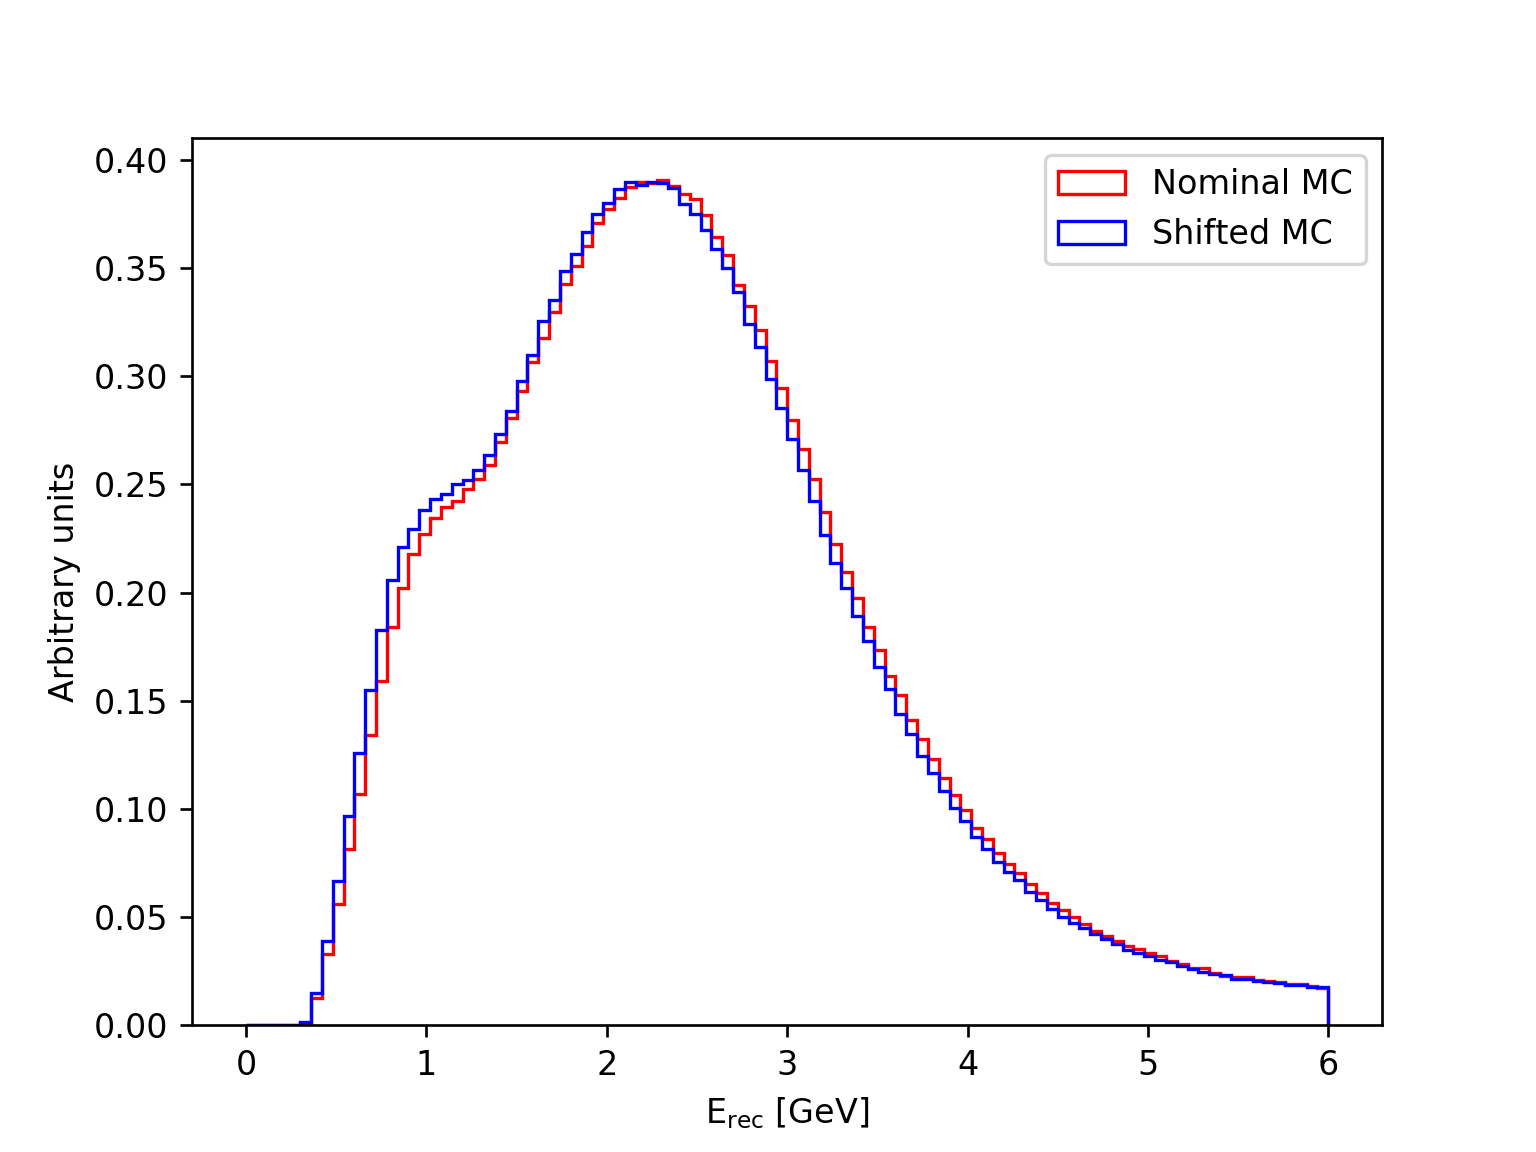
\includegraphics[width=0.45\textwidth]{hist_stop0_Erec_osc_noRW.png}

    %\label{fig:eproton_ndspec}
  }
  \subfloat[][$E_{res}$]{
    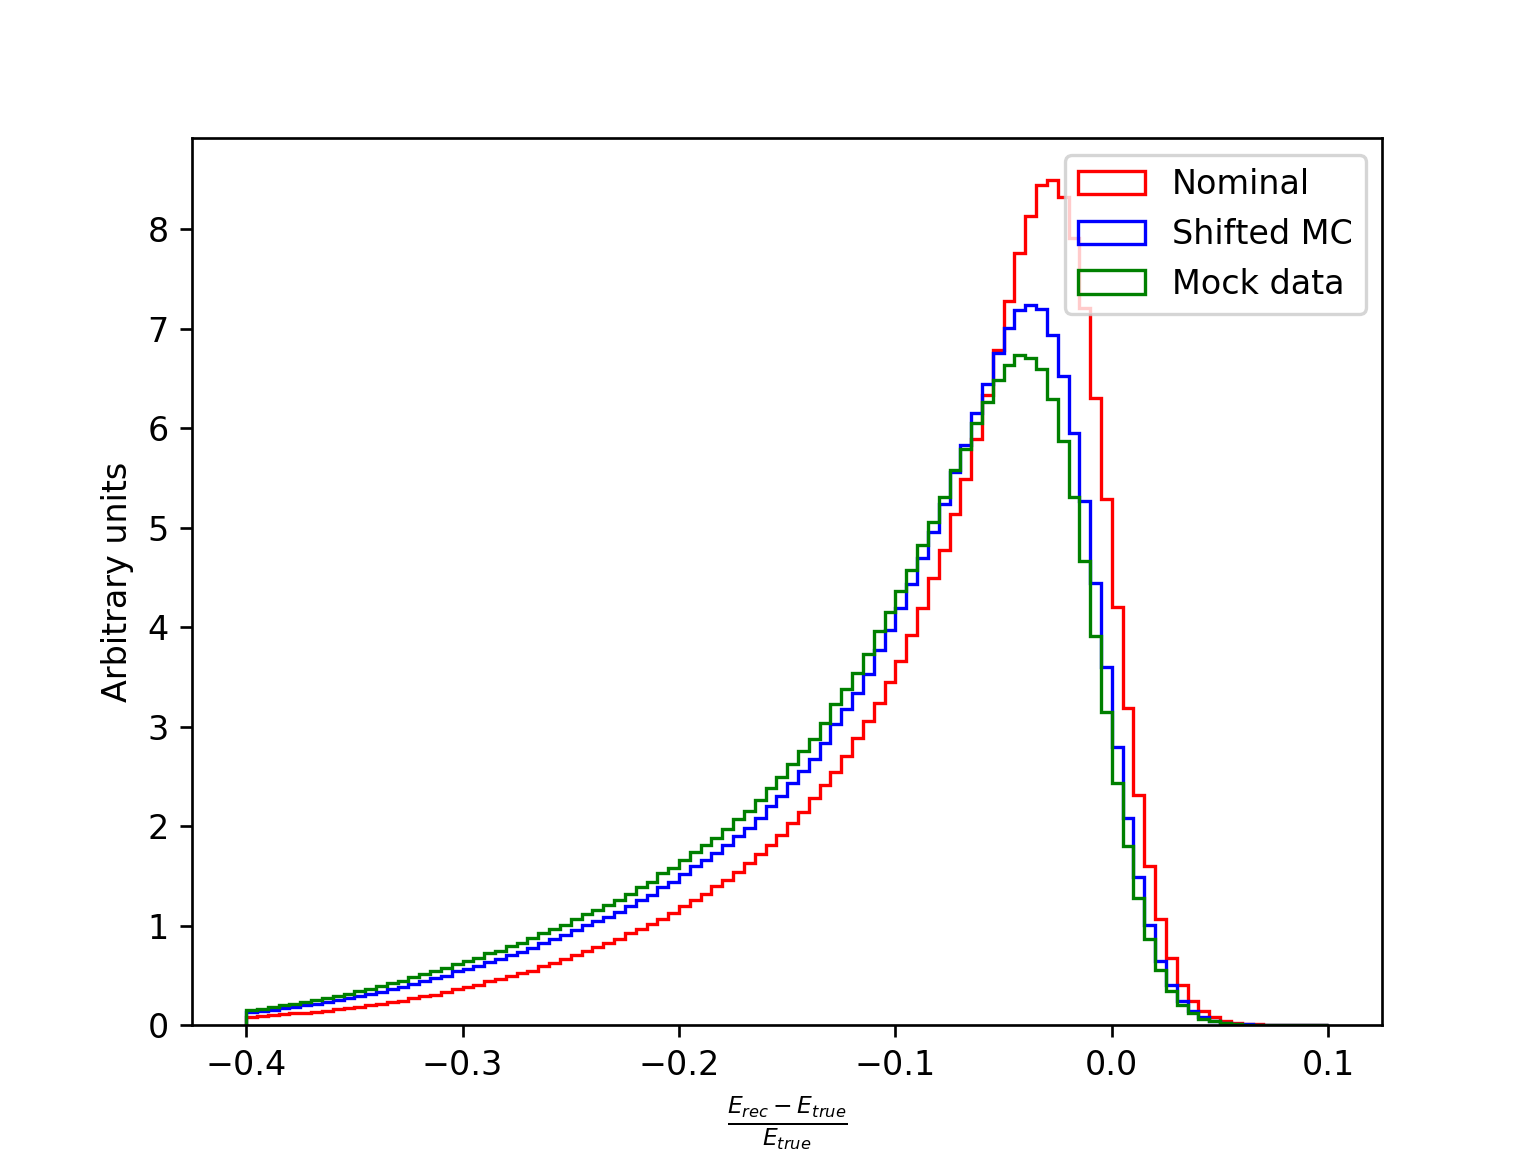
\includegraphics[width=0.45\linewidth]{FHC_Enu_Erec_fracDiff1D_m20pcProtonE.png}
    %\label{fig:eproton_enures}
  }
\end{dunefigure}





\begin{dunefigure}[$\nu_\mu$,$\nu_e$ at \dword{nd}]{fig:nuwro_study}
%  \centering
{Spectrum of $\nu_\mu$, $\nu_e$}
  \subfloat[][$Q^2$]{
    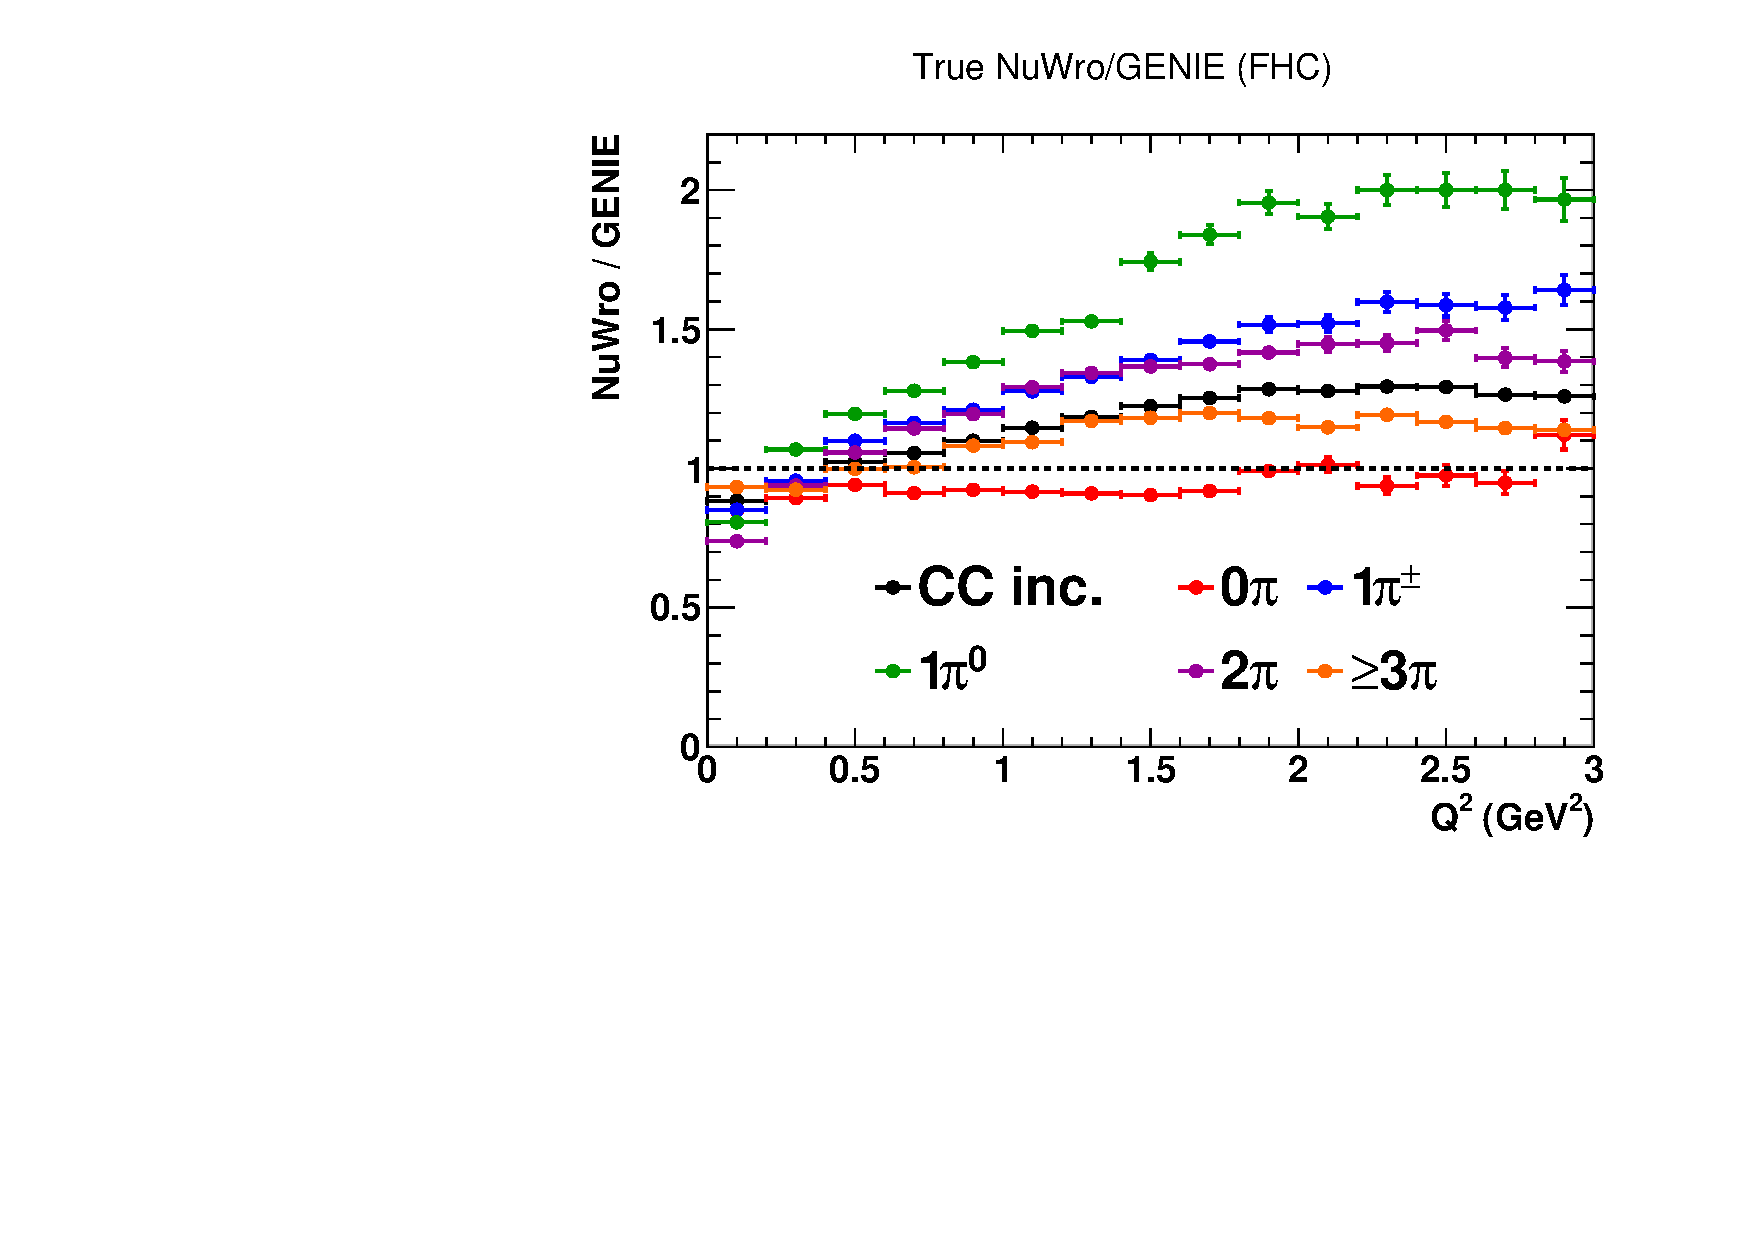
\includegraphics[width=0.45\textwidth]{graphics/PiStudyDataMCRatioTrueFHC.pdf}
    %\label{fig:eproton_ndspec}
  }
  \subfloat[][$\delta_{CP}$ ]{
    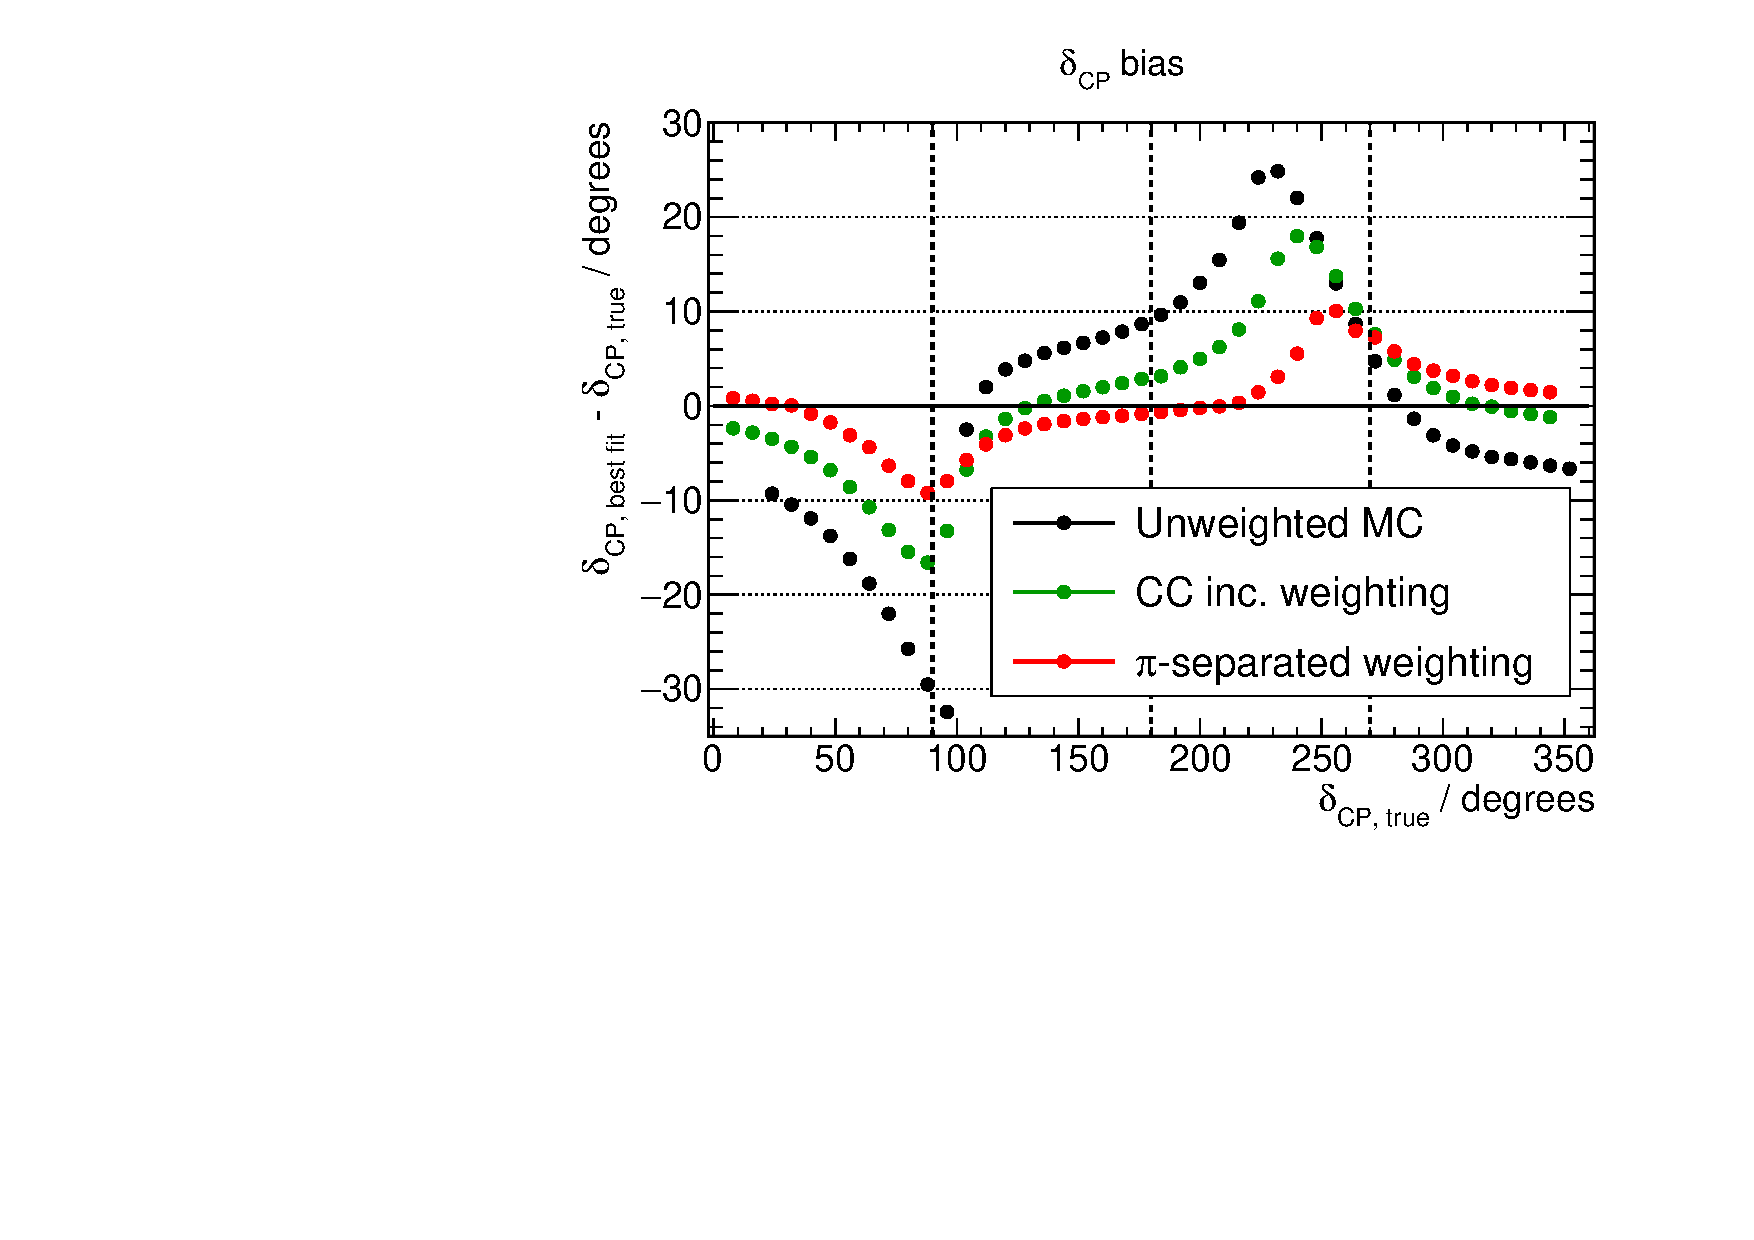
\includegraphics[width=0.45\linewidth]{graphics/PiStudyBiasWithGAr.pdf}
    %\label{fig:eproton_enures}
  }
\end{dunefigure}

%%%%%%%%%%%%%%
\subsection{Neutrino Interaction Modelling $\sigma_\beta$:}
All the properties of an interacting neutrino must be inferred from its outgoing particles. As a result, the modelling of neutrino-nucleus ($\nu-A$) interactions, particularly on argon in the case of \dword{dune}, is a critical element of the analysis. Since the oscillation parameters are extracted from the energy spectrum of neutrino interactions in each flavor, the modelling must provide the interaction cross section, summarizing the likelihood that the neutrino of a given flavor and energy interacts at all, as well as the details of the outgoing lepton and hadron systems, which are essential ingredients in understanding metrics like efficiencies/purities of the selected events and the resolution of quantities like the neutrino energy. For the hadron system in particular, the details of the particle content (particle type and kinematics) fundamentally impact the ionization and optical signal of the events, and thus the detector response is sensitive to this modelling regardless of whether the event selection and kinematic reconstruction chooses to use the details of the information or not.
Likewise, the modelling issues go beyond the determination of the $\nu-A$ cross section, but in include all aspects of modelling the $\nu-A$ interaction and the particles emerging from the target nucleus that impact the detector response. To that end, reference to ``$\sigma_\beta$'' and ``neutrino cross sections'' encompasses these issues, and not just ``cross sections'' narrowly defined. However, we exclude particle tracking and propagation effects in bulk media ({\em e.g.} LAr) which also  

It has been widely recognized that as accelerator-based neutrino oscillation experiments have increased in precision, commensurate improvements in neutrino-nucleus interactions are necessary to limit their impact on the systematic uncertainty budget. While the past decade has seen substantial progress both in measurements and theoretical/modelling, significant challenges remain both in defining a ``default'' model and adequately quantifing and propagating systematic uncertainties.

Among the concerns and challenges include:
\begin{itemize}
\item A handful of well-developed neutrino event generators and other models for $\nu-A$ interactions are available to the community. However, the generators have significant differences in the predicted properties of the $\nu-A$ interactions, even when they employ similar underlying models.
\item There have been a few ``surprises'' in the form of significant deviations from model predictions resulting from physics processes that were not accounted for. One example is the excess of pionless $\nu_\mu$ charged current 
\item Theoretically, it is recognized that 

\end{itemize}

In each case
%Summary of Role of near detector in LBL physics
%Explain major a priori uncertainties in neutrino flux, neutrino interactions, detector response. Visit examples from NOvA %and T2K about how near detectors reduce uncertainties.
%Discussion on coupling/convolution of uncertainties.
%Discussion on “out-of-model” uncertainties with Genie/NuWRO and missing proton energy  examples as case studies. Past %experience and current state of knowledge suggests that such uncertainties are inevitable . . .  . we’re not dealing with %the Standard Model of particle physics.
%Figures: Reprise of standard plots (dCP/MO significance, theta23 precision). Bias in dCP from NuWRO/Genie study. Bias in %theta23, Dm2 from missing proton energy study.




%%%%%%%%%%%%%%%%%%%%%%%%%%%%
\section{The DUNE Collaboration and the DUNE-US Project}
\label{intro:collab-proj}

\fixme{You may want to change the title, but put the CDR-to-PDR-to-TDR explanation in this section along with some explanation of how it fits into the project}

%%%%%%%%%%%%%%%%%%%%%%%%%%%%
\section{Near Detector Reference Design}
\label{intro:refdes}
%Uncertainties (Flux, cross section, detector modelling)
%State overarching requirements, give rough sense of required overall systematic error.  
%Requirements
%List key measurements, purpose, and requirements.



%%%%%%%%%%%%%%
\subsection{PRISM}
\label{intro:refdes-prism}
%\fixme{I think it makes more sense to keep PRISM within the reference design rather than after it, no?}
%Quick overview of concept and applications, how to form pseudo-Gaussian beams, flux matching with oscillations. Reference %CDR for mathematical details.
%Plots: Pseudo-gaussian beam example, Flux matching example.



%%%%%%%%%%%%%%
\subsection{ND-LAr}
\label{intro:refdes-ndlar}

%%%%%%%%%%%%%%
\subsection{Cryostat}
\label{intro:refdes-cryostat}

%%%%%%%%%%%%%%
\subsection{TMS (or ND-Gar?)}
\label{intro:refdes-tms}





%%%%%%%%%%%%%%%%%%%%%%%%%%%%
\section{The LBNF Near Site Conventional Facilities}
\label{intro:lbnf}



%%%%%%%%%%%%%%%%%%%%%%%%%%%%
\section{Staging: The Day-One Detector}
\label{intro:staging}

%Revisit muon spectrometry requirements for ND-LAr interactions, sensitivity plots showing that first goals can be reached without ND-GAr.


%%%%%%%%%%%%%%%%%%%%%%%%%%%%
\section{The DUNE-US Project Organization and Responsibilities}
\label{intro:collab-proj}



%%%%%%%%%%%%%%%%%%%%%%%%%%%%
\section{Summary of DUNE-US Scope}
\label{intro:us-scope}
